\chapter{Methodology}
\label{chp:methods}
This chapter presents the experimental methodology used throughout the subsequent experiment. This includes the collection of a large set of gait data and setup of a machine learning environment.

The chapter begins with a details of the development of a sensing system for human gait data. This is followed by work on collection of data and post processing. The final section contains details of the machine learning environment.

\section{Existing Datasets} % This should probably be part of the background
The quality of a data set is of key importance to the performance of any machine learning system trained from it.

\begin{table}[hbt]
    \centering
    \begin{tabularx}{\textwidth}{cYYYYY}
        \noalign{\hrule height 1.5pt}
        Dataset & Participants & Amputee Participants & \# Sensors & Type Sensors & Quantity \\ % What headings do we care about
        \hline
        OPPORTUNITY\cite{} & \\
        \noalign{\hrule height 1.5pt} \\
    \end{tabularx}
    \caption{Caption}
    \label{tab:my_label}
\end{table}

\cite{Cruciani2020} has lots of datasets - see Table 1
\cite{Micucci2017} Table 1
\cite{Vaizman2017} - Natural environment,
\cite{Garcia-Gonzalez2020}

\cite{Fu2021}

What sensors have people used? Where are the located? What activities have other performed? Environments tested in?

Reason why we need our own set


%------------------------------------------------------------------%
\section{Data Collection Hardware}
To collect a new set of first hand gait data a data collection system must be developed. The intention is for the data set to be made of real world unsupervised labelled data. Therefore the system must be simple to operate unaided, portable and non-intrusive. This section describes the solution that was developed to fulfil these requirements.


%--------------------------------------------------------
\subsection{Movesense Sensor}
The Suunto Movesense was chosen as the data collection platform. This is low cost (£70) \acrfull{cots} device containing a nine-axis \acrshort{marg} sensor, with built in heart rate monitor, temperature sensor and a \acrfull{ble} radio. The device is physically small weighing just ten grams and has the ability to be attached in numerous configurations. Figure \ref{fig:methods-movesense-sensor} shows the Movesense device.

\begin{figure}[hbt]
    \centering
    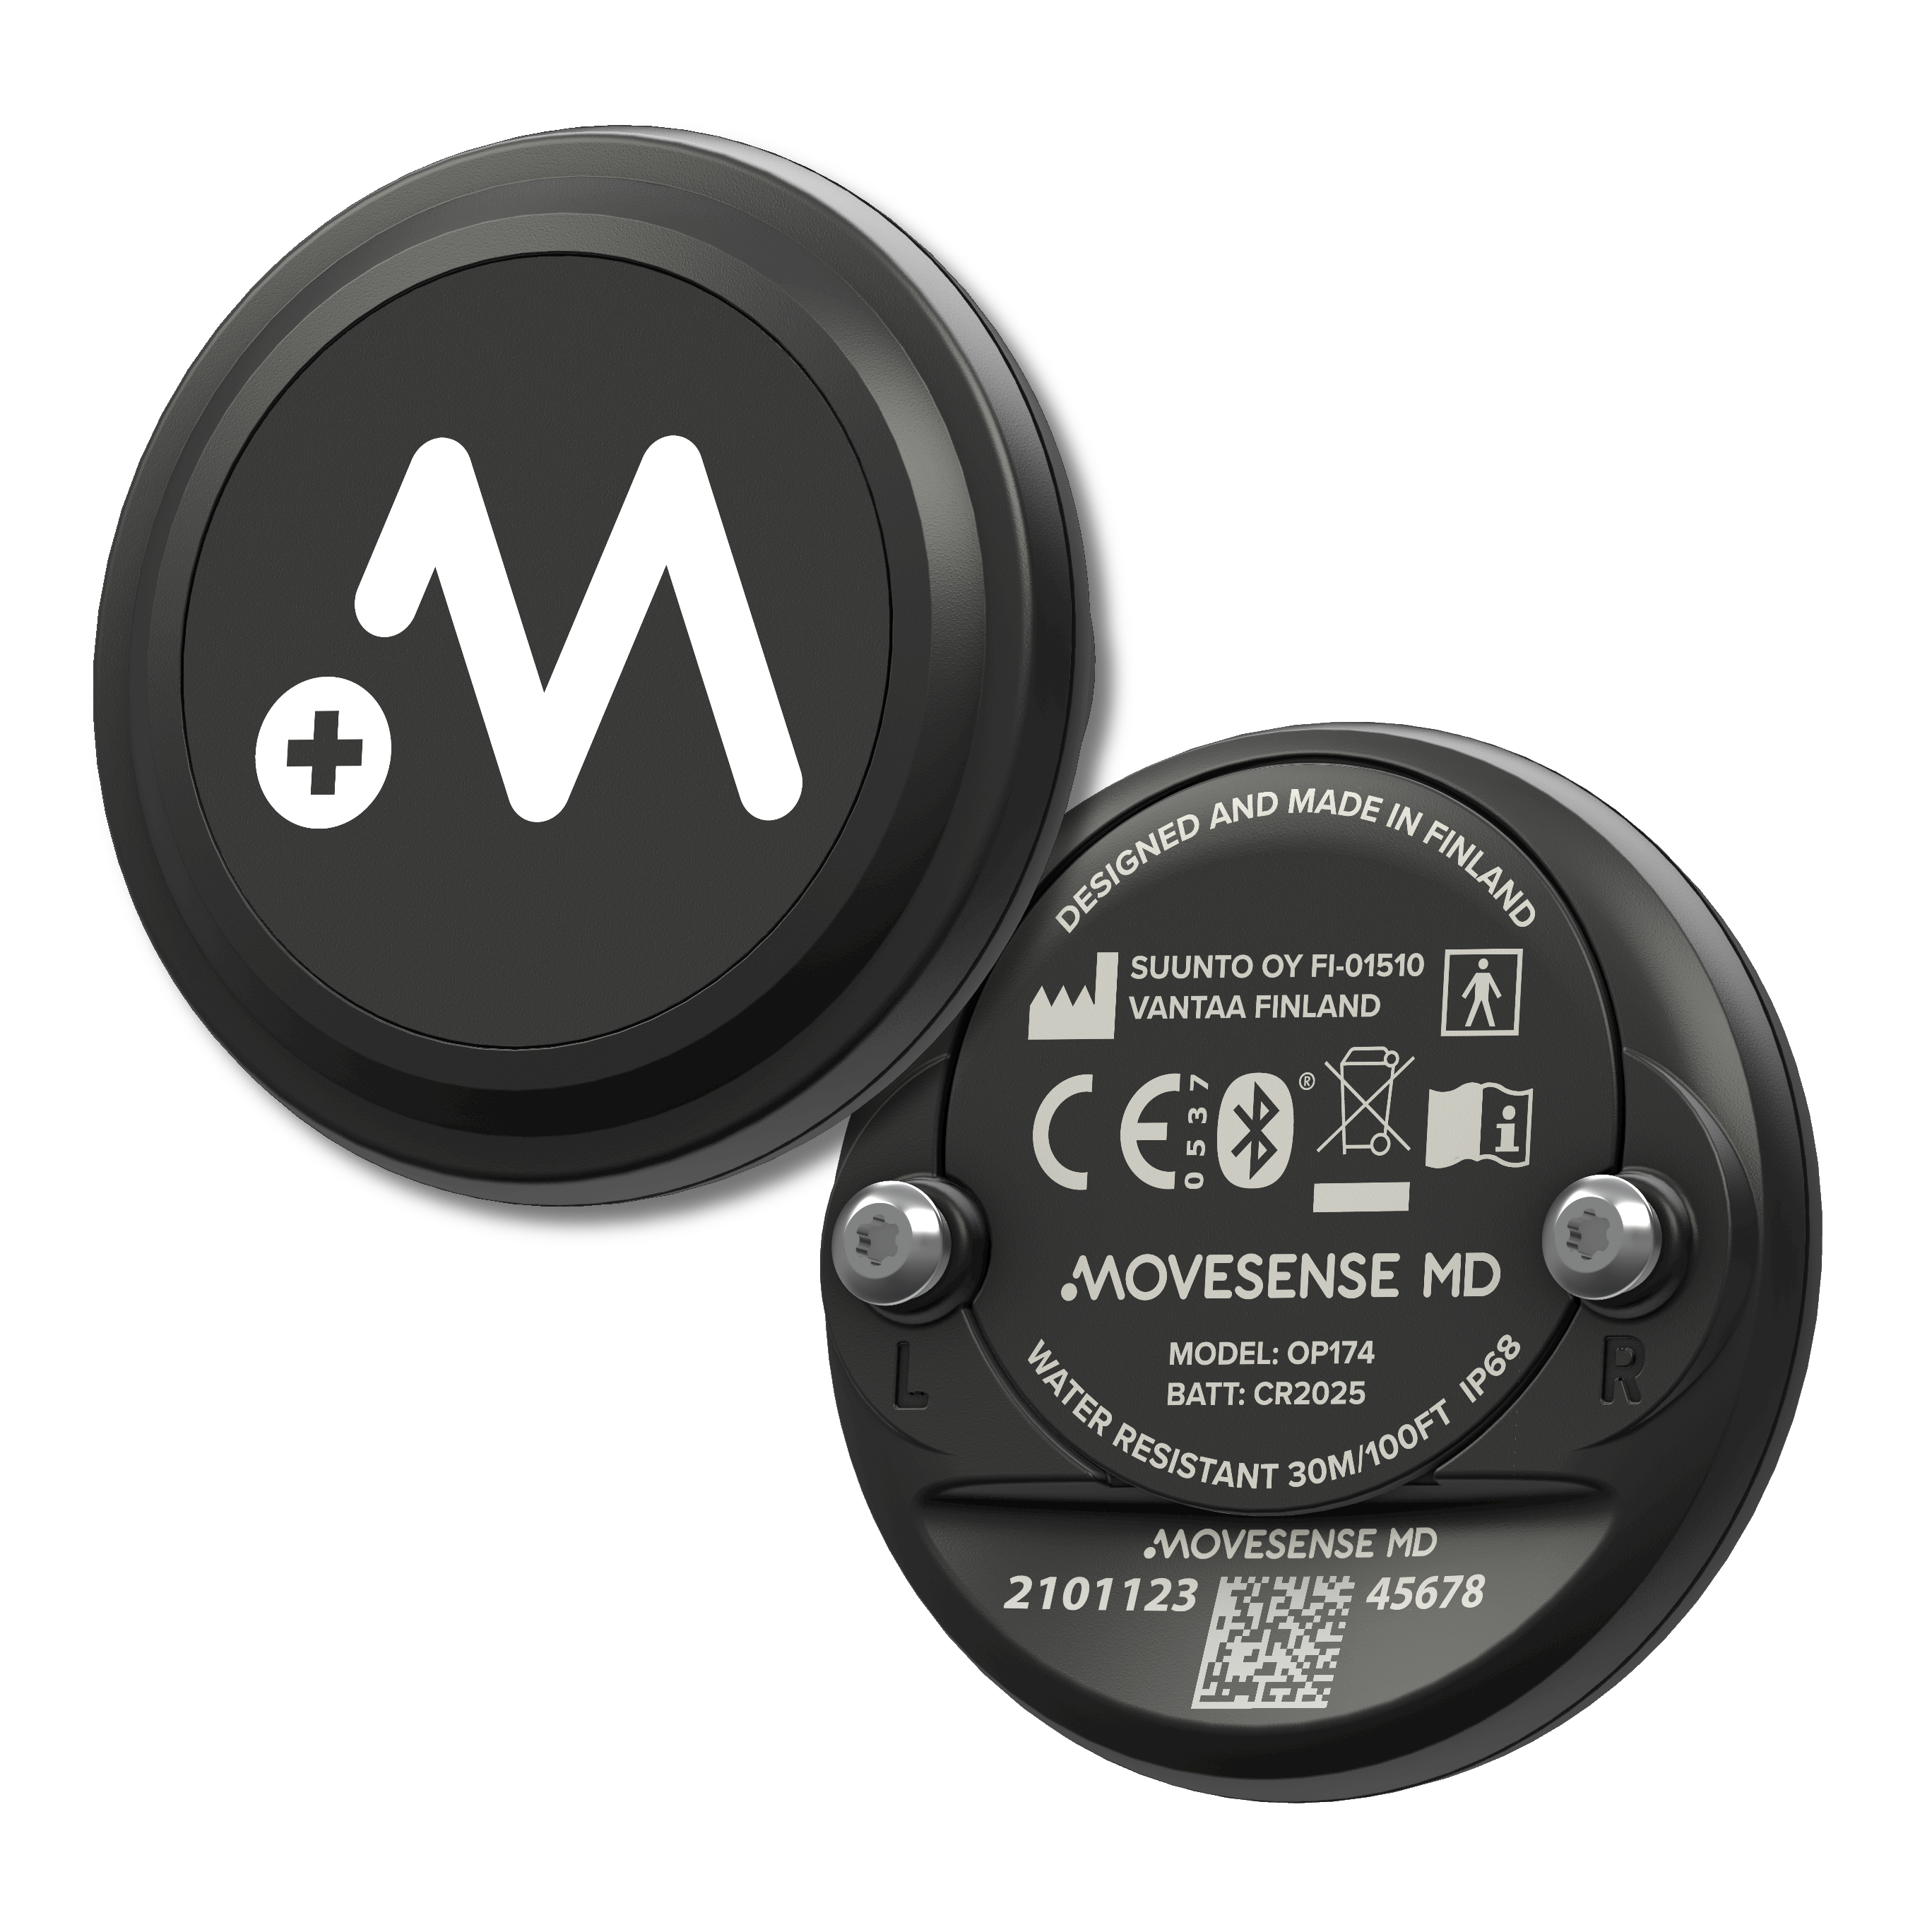
\includegraphics[width=0.5\textwidth]{content/3-Methods/Movesense-MD-front-and-back.png}
    \caption[Movesense Wearable IMU]{Movesense Wearable IMU\cite{}} % https://www.movesense.com/press/ - accessed 13-01-2022
    \label{fig:methods-movesense-sensor}
\end{figure}

The on-board \acrshort{marg} is factory calibrated with no additional sensor calibration required. The device is powered by a small coin cell battery that allows for continuous operation for multiple hours. A low power mode can be configured to significantly extend the usable lifetime.

Custom software can loaded using the \acrfull{sdk} provided by Suunto to configure the device in any manner required. A custom program was developed that transmits sensors readings over the \acrshort{ble} radio. The \acrshort{marg} output was transmitted at 100Hz, along with the latest heart rate and temperature sensor readings. The transmitted data was received by an Android phone running a custom data-logging application. Further details on these steps are presented in subsequent sections.

The software also implemented power management, placing the sensors in a ultra-low power state when inactive, as detected by low readings of the accelerometer, for more than 10 minutes. The devices could then be woken again by touching both rear contacts. This allowed the sensors to be shared with trial subjects without worry of replacing the batteries.

The device's rear contact also act as mounting point for attaching the device to a wide variety of sensors. These include heart rate and Velcro straps. Five sensors were attached to each participant in the following locations: on the inside of both ankles using an elastic Velcro strap, on~each hip using a clothes/belt clip and across the chest using a heart rate strap. The location of the sensors was selected to give wide coverage of body movements while providing easy, secure and non-invasive attachment to minimise discomfort and disruption to natural movement. Figure~\ref{fig:methods-movesense-sensor-locations} shows a subject wearing the five sensors.

\begin{figure}[hbt]
    \centering
    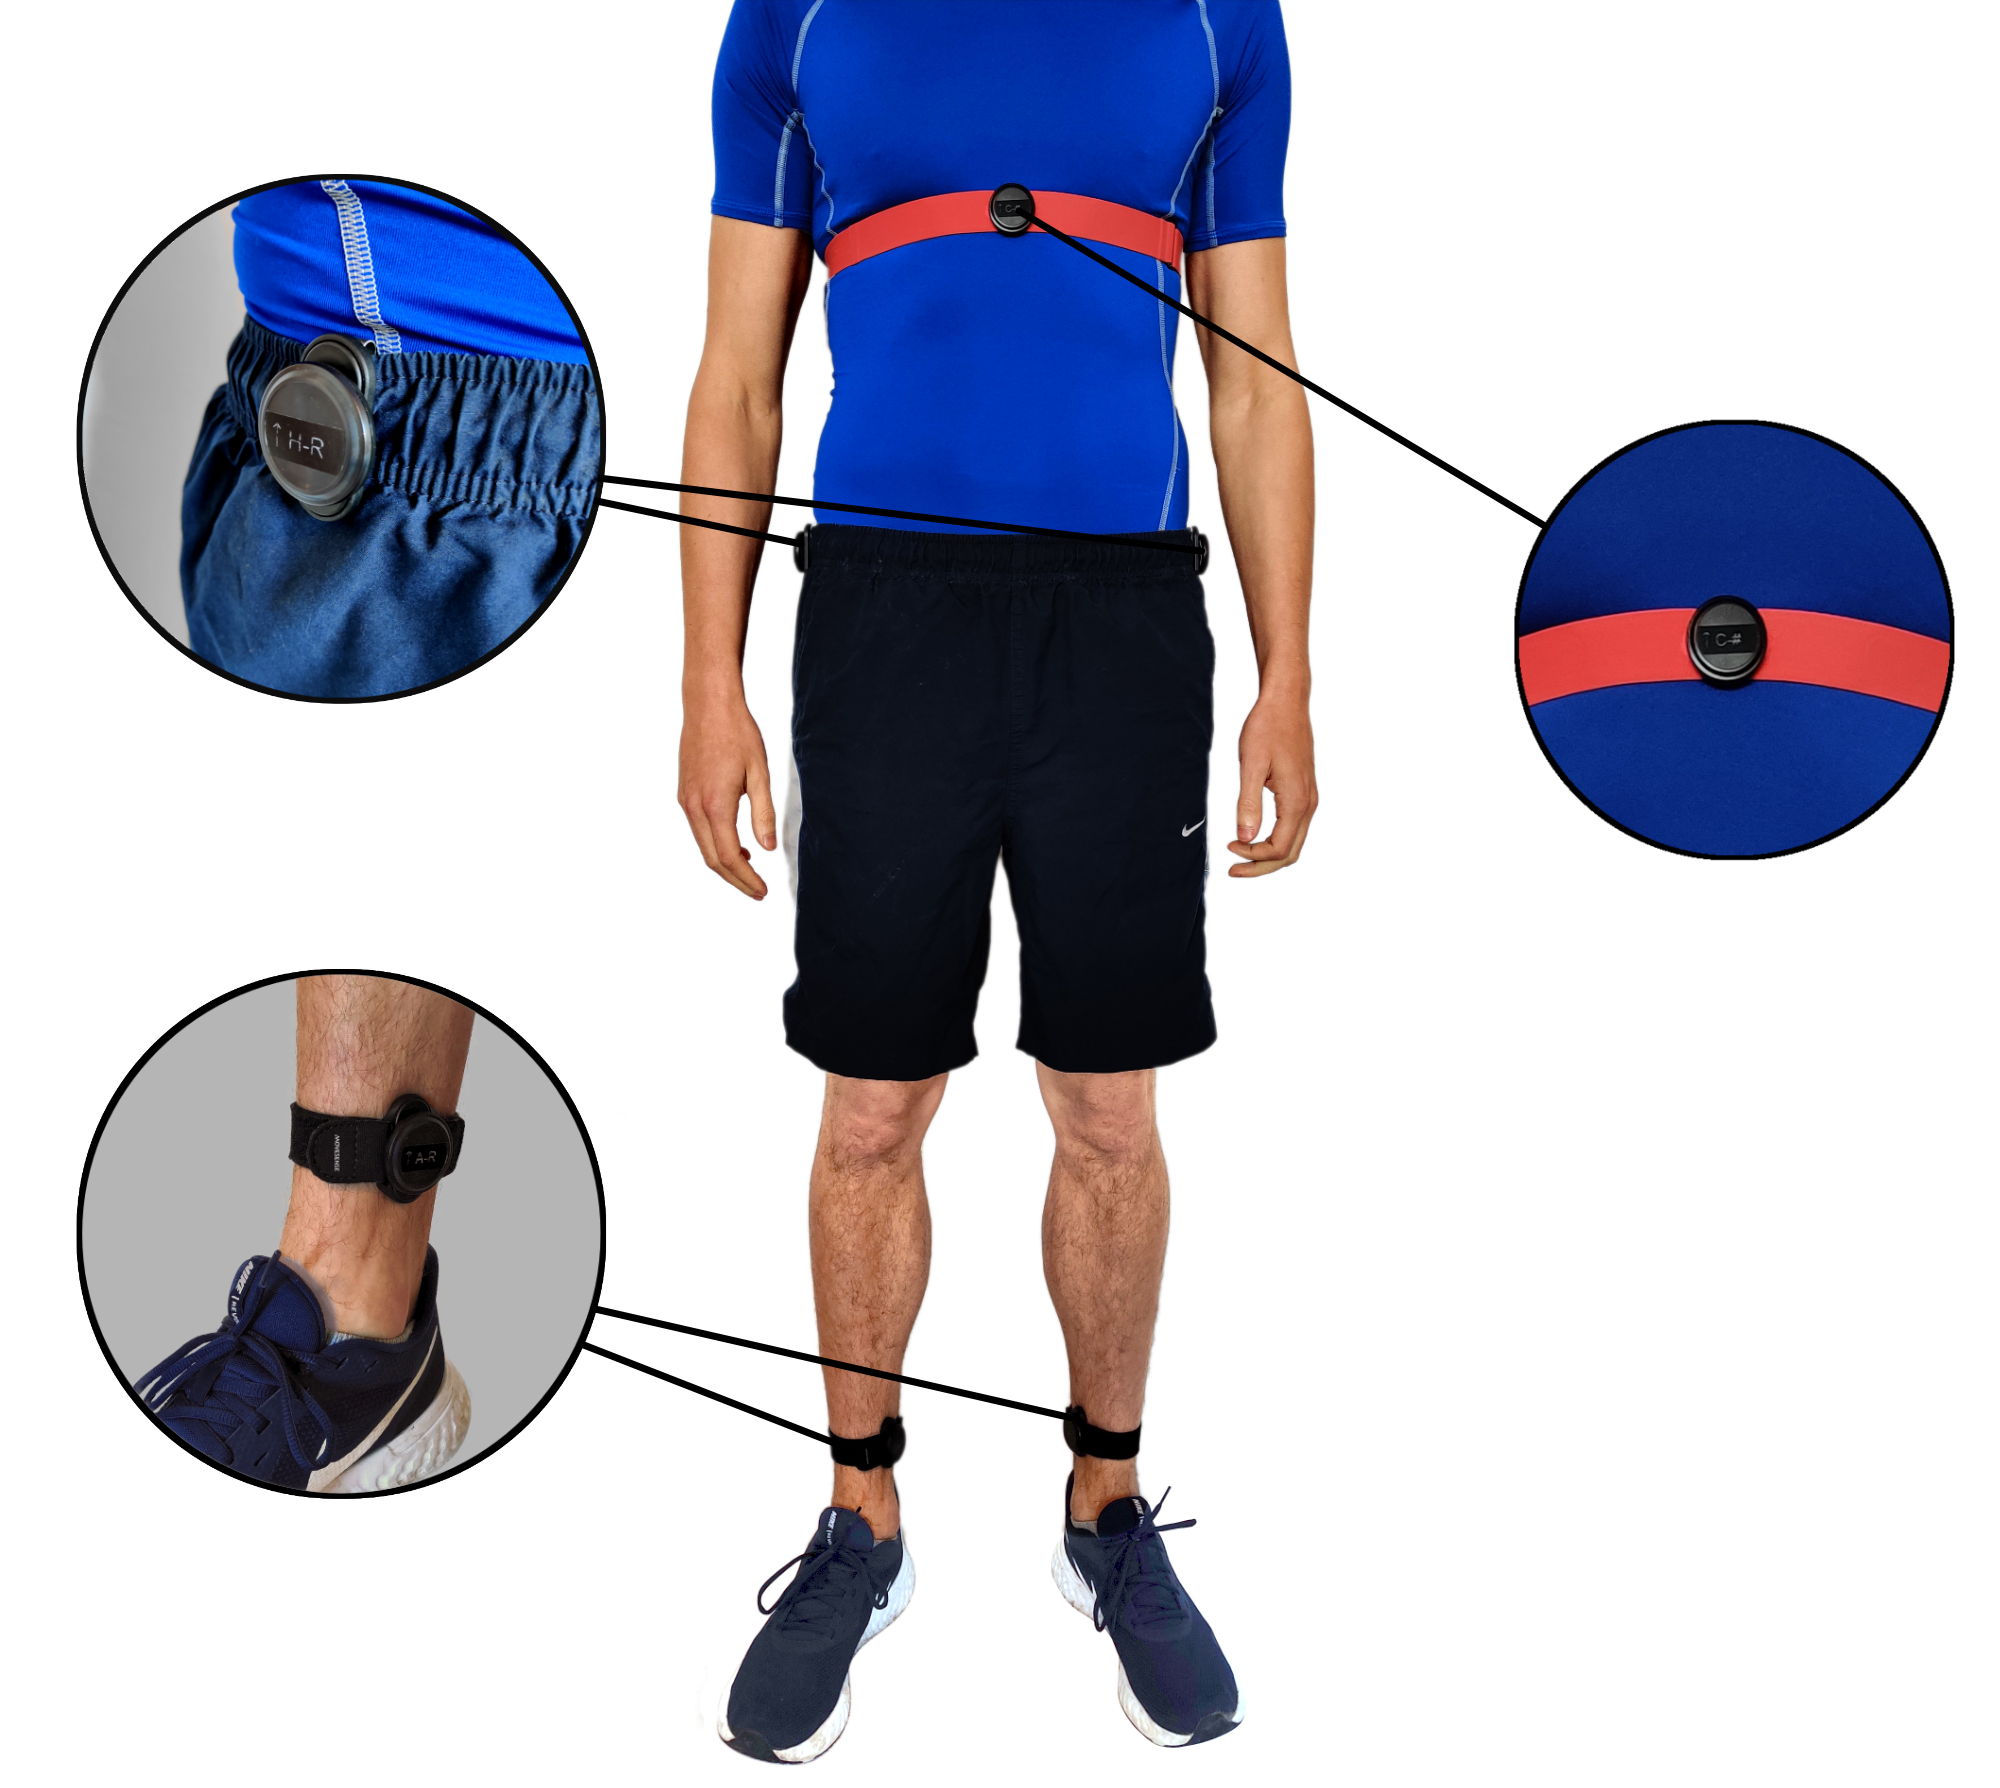
\includegraphics[width=0.6\textwidth]{content/3-Methods/sensor_locations.png}
    \caption{Movesense sensor attachment locations \cite{Sherratt2021}}
    \label{fig:methods-movesense-sensor-locations}
\end{figure}


%--------------------------------------------------------
\subsubsection{BLE Data Transmission} % How is sensor data transmitted 
\label{subsection:methods-on-sensor-compression}
Data is transmitted from each Movesense wirelessly to a smartphone using the built-in \acrfull{ble} radio transceiver. The process for preparing the sensor data for transmission is presented below.

A custom \acrfull{gatt} service was created that allows data packed to be pushed to a connected smartphone. Data pushing is done using the \acrshort{ble} notify mechanism. Data streaming starts when a notify state in the \acrshort{gatt} characteristic is set by the connected phone. Streaming then again when the notify state is cleared, either on disconnection or pragmatically clearing it. Data streaming is a high power state so this is on entered during recording.

Two limits restrict the data rate that the sensor can transmit. The maximum individual packet size and transmission rate. The maximum packet size is 155 bytes long. The practical limit of transmission rate is 15Hz, due to need to transmit concurrently from five sensors. These limits require multiple \acrshort{imu} samples to be transmitted per packet in order to achieve a real time 100Hz sample rate.

\acrshort{imu} data from the sensor is provided as a 32-bit floating point number. Therefore each full sample of the nine axis \acrshort{marg} sensor takes up 36 bytes. Uncompressed only four samples can be packed within the byte limit therefore compression of the data is required.

Compressing the data to a signed sixteen bit fixed point integer allow for eight measurements to be transmitted per packet. The compression is achieved by multiplying the original value by a scaling factor before typecast to a sixteen bit integer. This retains the sub-decimal accuracy while allowing for sufficient compression. Table \ref{tab:methods-imu-data-compression-factors} presents the sensor ranges, scaling factors and resultant accuracy of each sensor. As a sixteen bit integer values have a maximum range of $-32,768$ to $32,767$ clipping will occur if the typecast value of the sensors exceeds these limits. The scaling factor was therefore chosen as a balance between accuracy and output range. The output range requirement was calculated empirically.

\begin{table}[hbt]
    \centering
    \caption[Compression of sensor readings, scaling factors and resultant accuracies]{Compression of sensor readings, scaling factors and resultant accuracies. Force of Gravity (g), \acrfull{dps}, MicroTesla ($\mu T$)} % Fix caption units should be defined else where
    \label{tab:methods-imu-data-compression-factors}
    
    \begin{tabularx}{\textwidth}{Y|YYY}
        \noalign{\hrule height 1.5pt}
        \textbf{Sensor} & \textbf{Sensor Range} & \textbf{Scaling Factor} & \textbf{Accuracy} \\
        \hline
        Accelerometer & $\pm16 g$ & $256$ & $\pm0.039 g$ \\
        Gyroscope & $\pm2000 DPS$ & $32$ & $\pm0.031 DPS$ \\
        Magnetometer & $\pm5000\mu T$ & $1$ & $\pm1\mu T$ \\
        \noalign{\hrule height 1.5pt}
    \end{tabularx}
\end{table}

Once compressed eight \acrshort{marg} samples fit within one packet leaving eleven bytes available. A timestamp based on the internal sensor clock is transmitted as a 32-bit unsigned integer. Six further bytes are populated with the temperature, heart rate and R-R interval recording by the sensor. These were added for future use. As these values are only updated after a change in value the remaining byte is used as an update flag for each field. Figure \ref{fig:methods-ble-packet-structure} shows the full 155 byte transmission packet.

\begin{figure}[hbt]
    \centering
    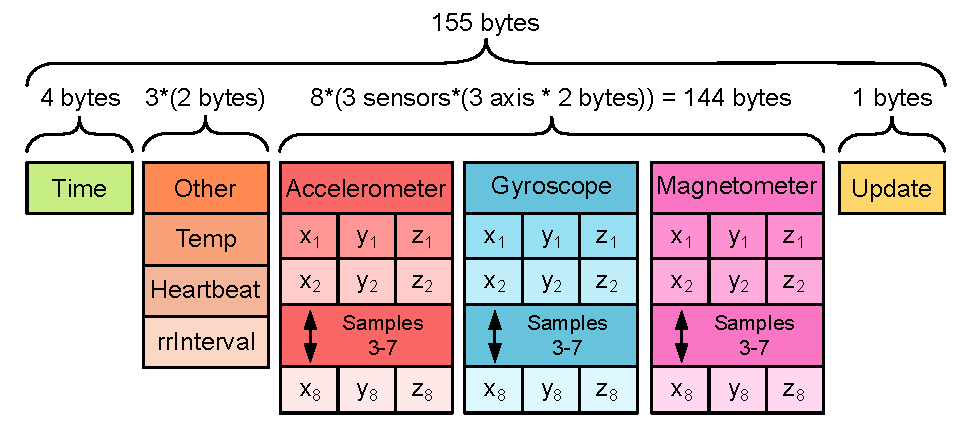
\includegraphics[width=0.9\textwidth]{content/3-Methods/BLE_Bytes_Packets.pdf}
    \caption[Movesense \glsentrylong{ble} transmission packet structure]{Movesense \acrlong{ble} transmission packet structure}    \label{fig:methods-ble-packet-structure}
\end{figure}


%--------------------------------------------------------
\subsection{Android Application}
The \acrshort{ble} data stream is received by a smart phone carried by the participant. The phone serves three purposes: to save the sensor data, to annotate the current activity, and to share annotated data with researchers. These three steps are described in more detail below. 

\subsubsection{User Interface}
The user interface of the application has been kept intentionally simple requiring minimal instruction to use. Figure \ref{fig:methods-app-user-interface} shows the application user interface in each of it's states.

\begin{figure}[hbt]
    \centering
    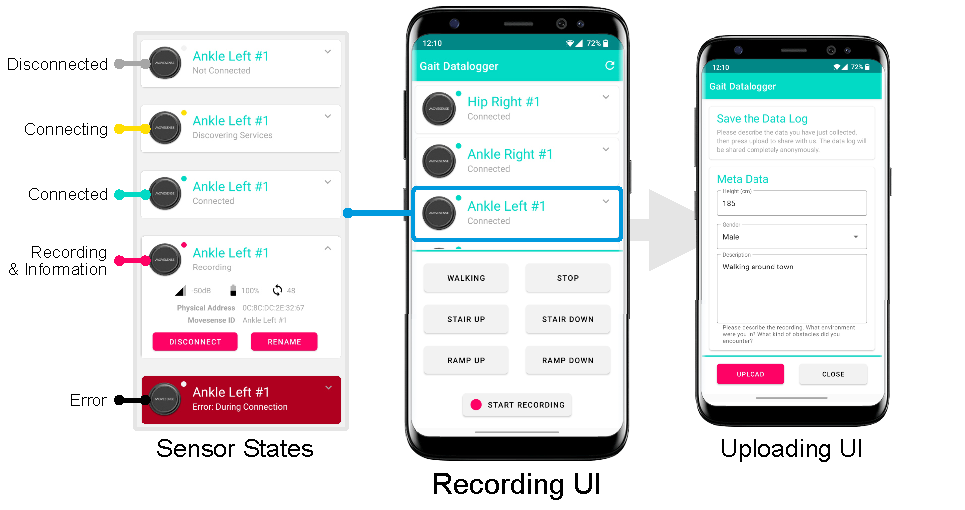
\includegraphics[width=\textwidth]{content/3-Methods/User_Interface.pdf}
    \caption{Data-logging Android application user interface}
    \label{fig:methods-app-user-interface}
\end{figure}

When the application is opened it attempts to connect automatically to detected sensor. This process can also be run manually by pressing the refresh button or dragging and releasing the list of devices. All detected devices show their current connection and activity states through a connection state icon and large status text. Any errors with sensors are clearly shown by highlighting the sensor in red and displaying error text.

To start and stop recording the subject pushes the `start recording' button at the bottom of the screen. All connected sensors start recording which should change their reported status to recording along with a red dot icon. The on board LED of each will also flash red to physically show it's state.

During recording a series of buttons at the bottom of application are used to annotate the current activities. Each time a button is pressed a log is created of both the activity name and current phone timestamp. Recording is halted by pressing the `stop recording` button. Once recording had finished the user is presented with an upload screen. This screen allows for metadata to be added and provides a system for sharing data with the researchers.

\subsubsection{Saving Sensor Data}
The android application is primarily responsible for forming a \acrshort{ble} connection to each sensor and saving the sensor data stream to a file that could be interpreted later. An illustration of the interactions between each aspect of the application is shown in Figure \ref{fig:methods-android-app}.

\begin{figure}[hbt]
    \centering
    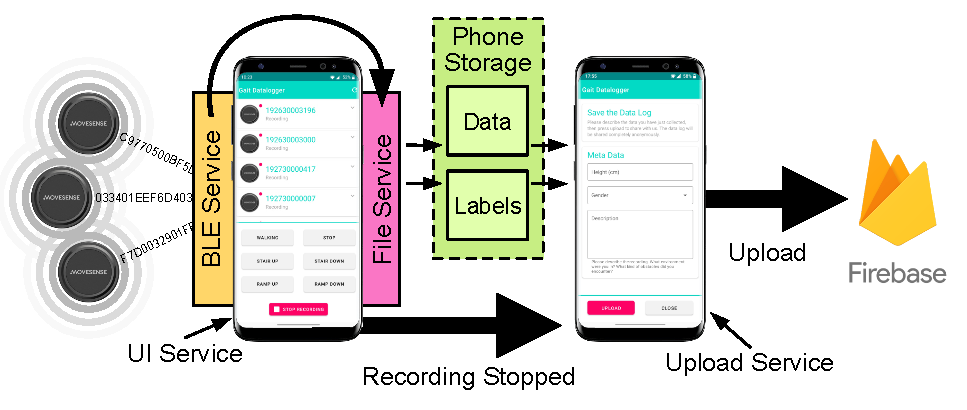
\includegraphics[width=0.9\textwidth]{content/3-Methods/Android_App.pdf}
    \caption{Data-logging Android App}
    \label{fig:methods-android-app}
\end{figure}

When the subject pressing the record button the notify state is set on each device starting data streaming. Received data is passed from the BLE service to the file saving service. This service creates plain text files locally on the phone. Each sensor message is saved on a new line along with the phone timestamp and MAC address of the sensor. The data message is saved as a hexadecimal representation of the data packet. All sensors are saved together in a single file with each line representing an individual data packet.

Once recording is finished the saved data can then be shared anonymously with the researchers using Google's Firebase cloud services. When the subject pressed uploads the locally saved files are uploaded to Google's cloud servers for later retrieval by researchers.


%------------------------------------------------------------%
\section{Data Collection}
\label{sec:methods-data-collection}
A large set of gait data is required develop \acrshort{ml} systems for classifying locomotive mode. This should be collected in real world unstructured environment so that common imperfections and disturbances are included. The data will be collected using the Movesense sensors described previously. The study received ethical approval from the University of Bath \acrfull{reach}, reference \textit{EP 19/20 003}.

%----------------------------------------------------------------
\subsection{Activities}
The following activities were selected, Walking, \acrfull{sa}, \acrfull{sd}, \acrfull{ra}, \acrfull{rd}) and Stopped. Labarri\`ere et al identified these as the most commonly investigated and they require no equipment or skill to perform~\cite{Labarriere2020}. These activities will be collected in the real world. Figure \ref{fig:methods-example-enviroments} shows examples of the environments that data was collected in.

% Pictures showing the variety of terrain %
\begin{figure}[!hbtp]
     \centering
     \begin{subfigure}[b]{\textwidth}
         \centering
         \begin{subfigure}[b]{0.32\textwidth}
             \centering
             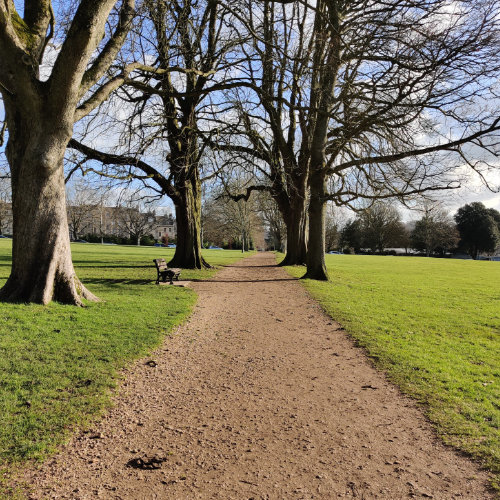
\includegraphics[width=\textwidth]{content/3-Methods/enviroments/flat_1_modified.jpg}
        \end{subfigure}
        \hfill
         \begin{subfigure}[b]{0.32\textwidth}
             \centering
             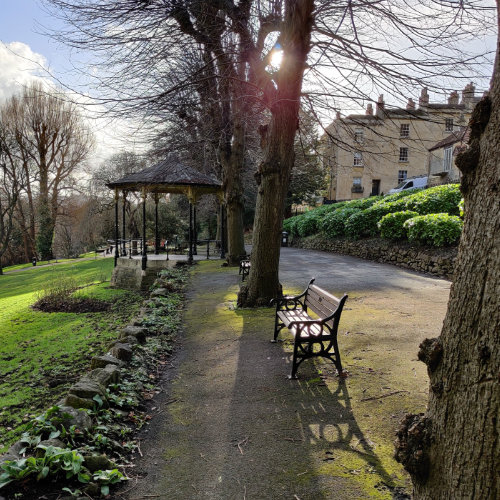
\includegraphics[width=\textwidth]{content/3-Methods/enviroments/flat_2_modified.jpg}
        \end{subfigure}
        \hfill
        \begin{subfigure}[b]{0.32\textwidth}
             \centering
             \includegraphics[width=\textwidth]{example-image-duck}
        \end{subfigure}
        \caption{Walking}
        \label{fig:methods-flat-example}
      \end{subfigure}
      \newline
      
      \begin{subfigure}[b]{\textwidth}
         \centering
         \begin{subfigure}[b]{0.32\textwidth}
             \centering
             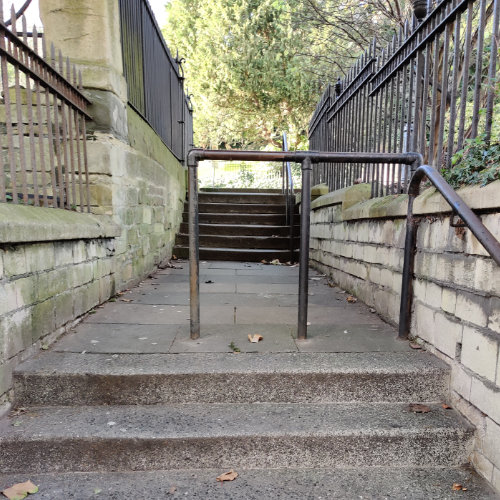
\includegraphics[width=\textwidth]{content/3-Methods/enviroments/stair_1_modified.jpg}
        \end{subfigure}
        \hfill
         \begin{subfigure}[b]{0.32\textwidth}
             \centering
             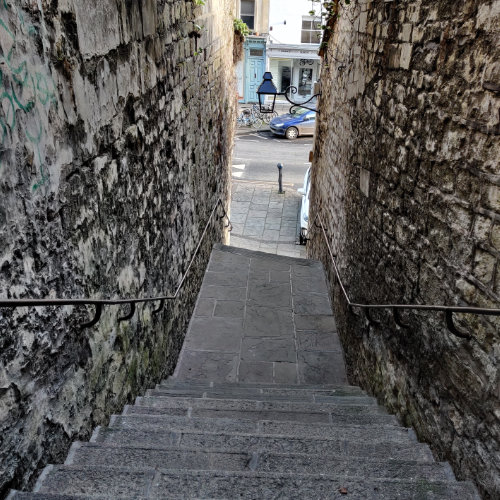
\includegraphics[width=\textwidth]{content/3-Methods/enviroments/stair_2_modified.jpg}
        \end{subfigure}
        \hfill
        \begin{subfigure}[b]{0.32\textwidth}
             \centering
             \includegraphics[width=\textwidth]{example-image-duck}
        \end{subfigure}
        \caption{Stairs}
        \label{fig:methods-stair-example}
      \end{subfigure}
      \newline
      
      \begin{subfigure}[b]{\textwidth}
         \centering
         \begin{subfigure}[b]{0.32\textwidth}
             \centering
             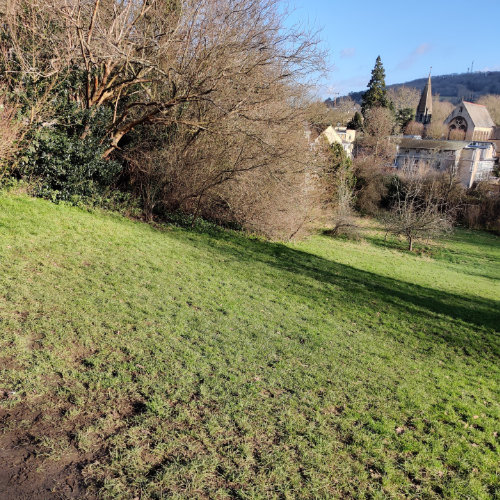
\includegraphics[width=\textwidth]{content/3-Methods/enviroments/ramp_1_modified.jpg}
        \end{subfigure}
        \hfill
         \begin{subfigure}[b]{0.32\textwidth}
             \centering
             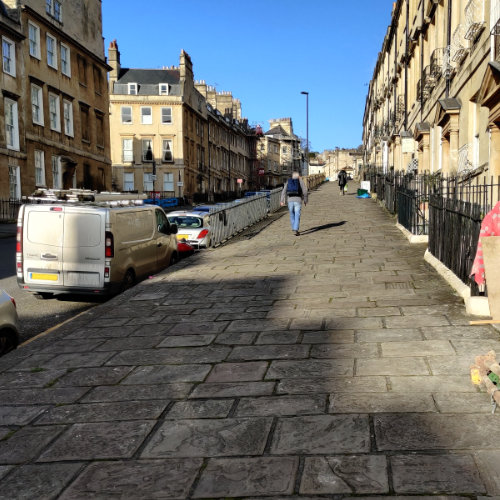
\includegraphics[width=\textwidth]{content/3-Methods/enviroments/ramp_2_modified.jpg}
        \end{subfigure}
        \hfill
        \begin{subfigure}[b]{0.32\textwidth}
             \centering
             \includegraphics[width=\textwidth]{example-image-duck}
        \end{subfigure}
        \caption{Ramp/Hill}
        \label{fig:methods-ramp-example}
      \end{subfigure}
    \caption{Example of data recording environments}
    \label{fig:methods-example-enviroments}
\end{figure}

%----------------------------------------------------------------
\subsection{Recording Procedure} % How were the subjects instructed to label data - press at first HS on new activity
Study subjects were provided with instructions on how to use the sensing equipment, along with general guidance on how to perform the experiment. Participants were instructed to walk around a varied environment with the sensor on while labelling the six activity classes. No further instructions on how the recording should be conducted were provided.

%----------------------------------------------------------------
\subsection{Summary of Data Collected} %TODO Expand on this section
A brief summary of the data collected over the course of this research is presented below.

Data was collected in three phases:
\begin{enumerate}
    \item Large number of non-amputee participants - limited data per participant
    \item Small number of non-amputee participants - extensive data per participant
    \item Data from amputees
\end{enumerate}

The first phase of data collection focused of collecting from a broad range of individuals in different environments. Table \ref{tab:methods-phase-1-data-summary} contains a summary of the data collected during the first phase of data collection. Data was collected from twenty-two participants of a wide variety of age (mean 29, std 10), gender (17 male, 5 female), and physique.

The second phase of data collection involved the collection of data from a smaller number of individuals but with a focus on collecting at least seven minutes of data for each activity. Table \ref{tab:methods-phase-2-data-summary} show a summary of the data collected during the second phase. Data was collected from three subjects, two males aged 25 and 27, and one female of age 26.

% Third round of data collection
The third stage of data collection focused on collecting data from amputees. Table \ref{tab:methods-phase-3-data-summary} contains a summary of the first hand data collected during this phase. The data was for one left trans-tibial individual.

\begin{table}[p]
    \centering
    \caption[Data samples of non-amputee data collected during the first phase of collection]{Summary of non-amputee data collected during the first phase of collection. (\acrfull{ra}, \acrfull{rd}, \acrfull{sa}, \acrfull{sd})}
    \label{tab:methods-phase-1-data-summary}
    %W---Walking, RA---Ramp Ascent, RD---Ramp Descent, SA---Stair Ascent, SD---Stair Descent, S---Stopped
    \begin{tabularx}{\textwidth}{c|YYYYYY}
       \noalign{\hrule height 1.5pt}
       \textbf{Subject ID} & \textbf{WALK} & \textbf{\glsentryshort{ra}} & \textbf{\glsentryshort{rd}} & \textbf{\glsentryshort{sa}} & \textbf{\glsentryshort{sd}} & \textbf{STOP} \\
       \hline
        01 & 34618 & 0 & 0 & 5349 & 5025 & 1281 \\
        02 & 13564 & 0 & 0 & 4614 & 4447 & 1020 \\
        03 & 5005 & 0 & 0 & 3633 & 2568 & 1587 \\
        04 & 32336 & 0 & 0 & 6045 & 5482 & 0 \\
        05 & 32525 & 0 & 0 & 6621 & 5767 & 0 \\
        06 & 37895 & 0 & 0 & 8424 & 5636 & 0 \\
        07 & 21843 & 0 & 0 & 14074 & 10873 & 0 \\
        08 & 38590 & 0 & 0 & 11036 & 17801 & 0 \\
        09 & 40384 & 0 & 0 & 10826 & 7953 & 0 \\
        10 & 37353 & 0 & 0 & 10812 & 8084 & 0 \\
        11 & 8341 & 0 & 0 & 1614 & 1566 & 0 \\
        12 & 9038 & 0 & 0 & 6273 & 4926 & 0 \\
        13 & 252022 & 48821 & 53735 & 18778 & 16220 & 16887 \\
        14 & 302440 & 18531 & 18305 & 10936 & 9581 & 73781 \\
        15 & 12249 & 0 & 0 & 1452 & 1929 & 3498 \\
        16 & 23729 & 0 & 0 & 5332 & 2578 & 1651 \\
        17 & 113222 & 2702 & 3754 & 3190 & 3949 & 19127 \\
        18 & 37352 & 0 & 0 & 3747 & 2565 & 1133 \\
        19 & 4990 & 0 & 0 & 1240 & 1245 & 0 \\
        20 & 3487 & 0 & 0 & 2383 & 3054 & 0 \\
        21 & 4806 & 0 & 0 & 2551 & 190 & 206 \\
        22 & 9033 & 3274 & 3630 & 982 & 938 & 856 \\
        \hline
        \textbf{Total} & 1075111 & 73328 & 79426 & 139915 & 122378 & 121027 \\
        \noalign{\hrule height 1.5pt}
    \end{tabularx}
\end{table}

\begin{table}[p]
    \centering
    \caption[Data samples of non-amputee data collected during the second phase of collection]{Data samples of non-amputee data collected during the second phase of collection. (\acrfull{ra}, \acrfull{rd}, \acrfull{sa}, \acrfull{sd})}
    \begin{tabularx}{\textwidth}{c|YYYYYY}
       \noalign{\hrule height 1.5pt}
       \textbf{Subject ID} & \textbf{WALK} & \textbf{\glsentryshort{ra}} & \textbf{\glsentryshort{rd}} & \textbf{\glsentryshort{sa}} & \textbf{\glsentryshort{sd}} & \textbf{STOP} \\
       \hline
       01 & 462446 & 141268 & 139786 &59685 & 44024 & 62397 \\
       03 & 291213 & 77508 & 59157 & 48695 & 50210 & 157867 \\
       09 & 368090 & 115299 & 82980 & 49530 & 51698 & 60605 \\
       \hline
       \textbf{Total} & 2100308 & 404127 & 364574 & 277250 & 252494 & 363669 \\
       \noalign{\hrule height 1.5pt}
    \end{tabularx}
    \label{tab:methods-phase-2-data-summary}
\end{table}
% Amputee data
\begin{table}[p]
    \centering
    \caption[Data samples of first hand amputee data collected during the third phase of collection]{Data samples of first hand amputee data collected during the third phase of collection. (\acrfull{ra}, \acrfull{rd}, \acrfull{sa}, \acrfull{sd})}
    \begin{tabularx}{\textwidth}{c|YYYYYY}
       \noalign{\hrule height 1.5pt}
       \textbf{Subject ID} & \textbf{WALK} & \textbf{\glsentryshort{ra}} & \textbf{\glsentryshort{rd}} & \textbf{\glsentryshort{sa}} & \textbf{\glsentryshort{sd}} & \textbf{STOP} \\
       \hline
       A1 & 38114 & 6159 & 7194 & 2872 & 2450 & 11763 \\
       \noalign{\hrule height 1.5pt}
    \end{tabularx}
    \label{tab:methods-phase-3-data-summary}
\end{table}

% % Discussion about collected data
% What is unique about our data set
% \begin{itemize}
%     \item Unsupervised (no researcher bias in activity pattern) - subject Provided with sensors, app and basic instructions of how to setup and label data
%     \item Wide range of different natural environments and terrain
%     \item Large number of people
%     \item Comparable data from an amputee
% \end{itemize}

% Systematic issues with the data set
% \begin{itemize}
%     \item Poorly distributed classes - real life distribution of activities is not even. Walking and hills/ramps are far more prevalent than stairs.
%     \item Label noise due to likely inconsistencies between individuals when collecting data
%     \item Different amounts of data for different participants
% \end{itemize}


%------------------------------------------------------------------%
\section{Data Post-Processing}
The raw data must be transformed in order that it can be used in a machine learning environment. Within this sections the methods used to accomplish this transformation are detailed.

% Terminology
The data collected can be described by the following hierarchical structure shown in Figure \ref{fig:methods-data-hierachy}. For each participant a series of gait data is recorded. Each recording is live annotated using the android app. Recordings potentially contain different distributions of activities from different environments. Each continuous period of an activity label is an episode of data. So a recording is made up of a series of contiguous episodes of data. The period at the end of episode and start of the next is the transition period between activities. This is represented as a discrete change but in reality would be a smooth easing between locomotive modes.

\begin{figure}[hbt]
    \centering
    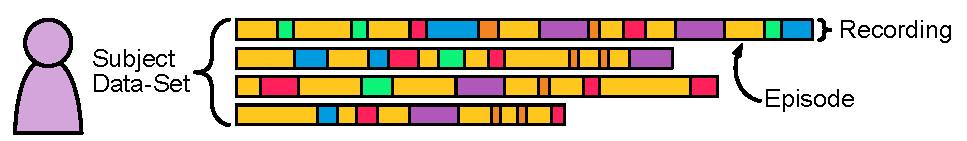
\includegraphics[width=0.9\textwidth]{content/3-Methods/Data_Terminology.pdf}
    \caption{Hierarchical structure of the data recordings and terminology}
    \label{fig:methods-data-hierachy}
\end{figure}

%Issues with the data
To prepare the data for \acrshort{ml} and address systematic issues with the data two \acrfull{etl} scripts were developed. An \acrshort{etl} is a common technique in data science for copying data from one or more source to a new destination where a different representation is required. A \acrshort{etl} script written in Matlab 2019b is used to transform the sensor data from it's raw form to \acrshort{csv} files that can be imported into a Python environment. A second \acrshort{etl} script written in Python 3.7 then prepare the data for loading into a machine learning environment. A more detailed description of these two scripts is presented in the remainder of this section.

\subsection{Sensor Data ETL}
\label{subsec:sensor-ETL}
The sensor data \acrshort{etl} script transforms the raw sensor data into \acrshort{csv} tables that are easily importable into Python. The overall process is illustrated in Figure \ref{fig:methods_sensor_ETL}. Further detail of ach step \acrshort{etl} is described below.

\begin{figure}[hbt]
    \centering
    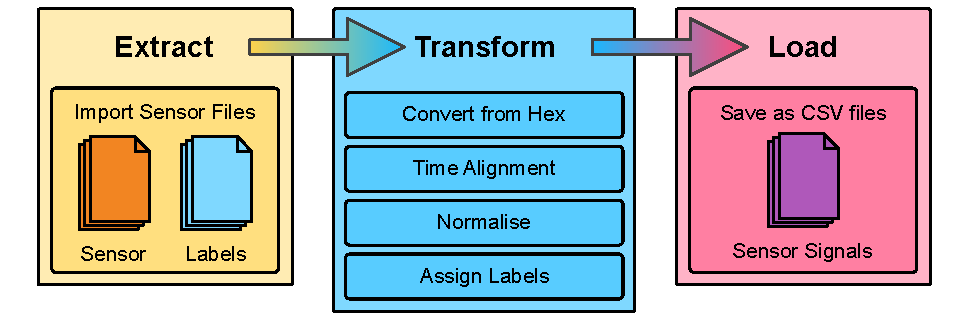
\includegraphics[width=0.9\textwidth]{content/3-Methods/Sensor_ETL.pdf}
    \caption{Flow Diagram of Sensor Data \acrshort{etl} process}
    \label{fig:methods_sensor_ETL}
\end{figure}

\subsubsection{Extract} % Extract - retrieving data from source
Data is saved in individual directory for each participant and a sub-directory for each recording session. Within each sub-directory three files are store, a data file, label file and meta-data file. The meta data does not form part of the \acrshort{etl} output. The three files contain the following:
\begin{itemize}
    \item \textbf{Data File} -- Hexadecimal encoded binary sensor data along with the mobile phone timestamp at which it was received.
    \item \textbf{Label File} -- Plain text activity labels with timestamps of the activity start (the point at which the application button was pressed)
    \item \textbf{Meta File} -- Notes about the recording including the participant height, gender and a brief unstructured description of the recording.
\end{itemize}

Each sub-directory is opened and processed one at a time in order of recording date.

\subsubsection{Transform}
% Transform
The sensor data is store as a hexadecimal string, with each pair of characters representing one byte of the sensor transmission data. The first operation is converting each pair of characters into it's binary form. Then sets of binary values are typecast to integer values before apply the appropriate scalars to convert back to their original 32-bit floating point representation. This is the reverse of the on sensor compression described previously.

Each line of sensor data contains the Physical/MAC address of the sensor. This is used to split the combined data file into individual sensors. Before combining the individual sensors into a single data table any inconsistency between the devices needs to be accounted for.

The sensors do not have on-board real-time clocks with the sensor timestamp is based upon their internal clock oscillator. There is sufficient variation between these that clock drift between sensors must be accounted for. To calculate a correction for the long term drift the message timestamp is compared to the smartphone's clock. This drift is assumed to be linear therefore linear regression can used be to determine a correction offset and gain. Figure \ref{fig:methods-clock-drift-correction} shows an example of drift correction.

\begin{figure}[hbt]
    \centering
    \begin{subfigure}{0.45\textwidth}
         \centering
         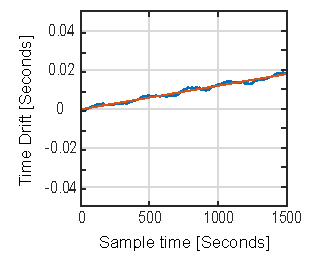
\includegraphics[width=0.95\textwidth]{content/3-Methods/Clock_Drift.pdf}
         \caption{Before correction}
    \end{subfigure}
    \begin{subfigure}{0.45\textwidth}
         \centering
         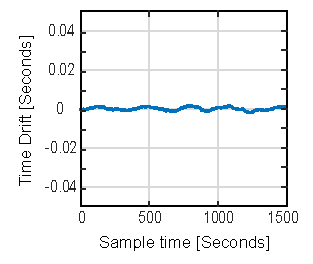
\includegraphics[width=0.95\textwidth]{content/3-Methods/Clock_Drift_Corrected.pdf}
         \caption{After correction}
    \end{subfigure}
    \caption{Example of sensor clock drift correction}
    \label{fig:methods-clock-drift-correction}
\end{figure}

Each data packet contains eight sensors readings, but only one timestamp. Therefore the timestamps for the each individual reading needs to be augmented. This is done by assuming the data is recorded at the recording frequency.

Finally the data is re-sampled to exactly 100Hz to ensure data for each sensors aligns correctly. This was necessary as due to inconsistent in sensor clocks the actual device sample rate varied by a couple of Hertz. Re-sampled is performed using the built in Matlab re-sampling function. This uses a spline function to calculate the interpolated value. At this point the individual sensors can be combine into a single data table.

Among these, data normalisation is an essential pre-processing step which involves the transformation of features in a common
range so that greater numeric feature values cannot dominate the smaller numeric features values. The main aim is to minimize the bias of those features whose numerical contribution is higher in discriminating pattern classes.

Data normalisation has been shown to improve the performance of \acrshort{ml} models by ensuring features with greater numerical values cannot dominate smaller features\cite{Singh2020}. Normalisation is performed on a per recording basis maintaining the changes in magnitude that occur when changing between activities. Each channel of data is normalisation independently. The values for scaling and offset would need to specified on a per user basis for a physical system.

The last step is applying activity labels to the data table. The data labels recorded in the label file are aligned based on the smartphone's clock. Each row in the data table is given a label based on the last activity label encountered.

\subsubsection{Load}
Two saving options were employed:
\begin{itemize}
    \item Saving the complete recording as a single file
    \item Splitting the recording up into different files for each episode of an activity
\end{itemize}

The data tables are exported as \acrfull{csv} files, with files for each participant stored in separate folders. Basic statistics about each file are also generated, including number of samples of each activity and step count.

%--------------------------------------------%
\subsection{Machine Learning ETL}
\label{subsec:ML-ETL}
The second \acrshort{etl} script ingests the \acrshort{csv} data files previously generated and converts and prepares them for loading into a Tensorflow \acrshort{ml} environment. Tensorflow requires three sets of data, train, test, and validation, each presented as a set of data inputs along with a corresponding expected output. The \acrshort{etl} script is written in Python 3.8. A flow diagram of the \acrshort{etl} process is shown in Figure \ref{fig:methods_ml_ETL} shows the process, below additional detail for each step is presented.

\begin{figure}[hbt]
    \centering
    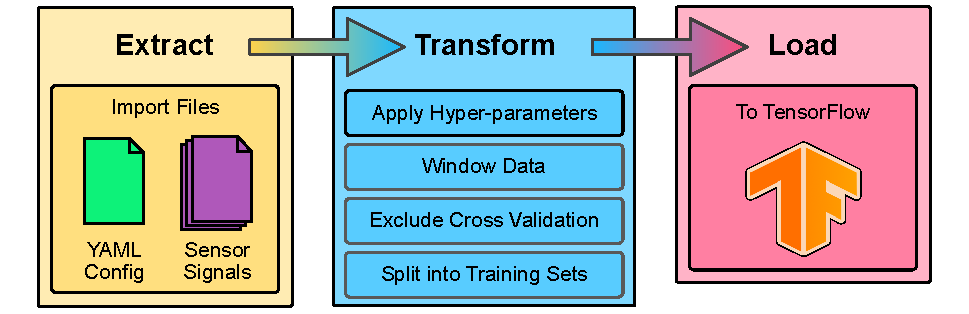
\includegraphics[width=0.9\textwidth]{content/3-Methods/ML_ETL.pdf}
    \caption[Flow Diagram of the \glsentrylong{ml} ingest \glsentryshort{etl} process]{Flow Diagram of the \acrlong{ml} ingest \acrshort{etl} process}
    \label{fig:methods_ml_ETL}
\end{figure}

% Export
\subsubsection{Extract}
The \acrshort{etl} script accepts a \acrshort{yaml} configuration file. This files contains the configuration for the machine learning experiment being run. This allow experiments to be replaced quickly as the \acrshort{yaml} files can be stored with the input data and results. The \acrshort{etl} script also supports a \acrshort{yaml} file that specifies a set of values for a parameter. This allows the \acrshort{etl} script to implement hyper-parameter sweeping.

The extract imports the \acrshort{csv} files previously generated from a directory specified in the configuration file using the Python library Pandas. This produces Pandas data tables which are stored in memory with a mapping to their associated participant and activity where applicable.

 
\subsubsection{Transform}
Hyper-parameters extracted from the \acrshort{yaml} file are use across all aspects of the transformation process to define constants.

The \acrshort{yaml} setup file specifies the columns of data that are required, for example \textit{right-ankle-gyro-y}. These data columns are extracted from the Pandas data tables with the remaining data discarded.

To generate the data windows rows of data equal to the specified window size are selected and copied to form new Pandas data tables. This starts at the beginning of the data table with the starting index incremented forward by a specified skip value for each new window. This results in a set of overlapping windows. Figure \ref{fig:methods-data-window-generation} illustrates the data windowing process.

\begin{figure}[hbt]
    \centering
    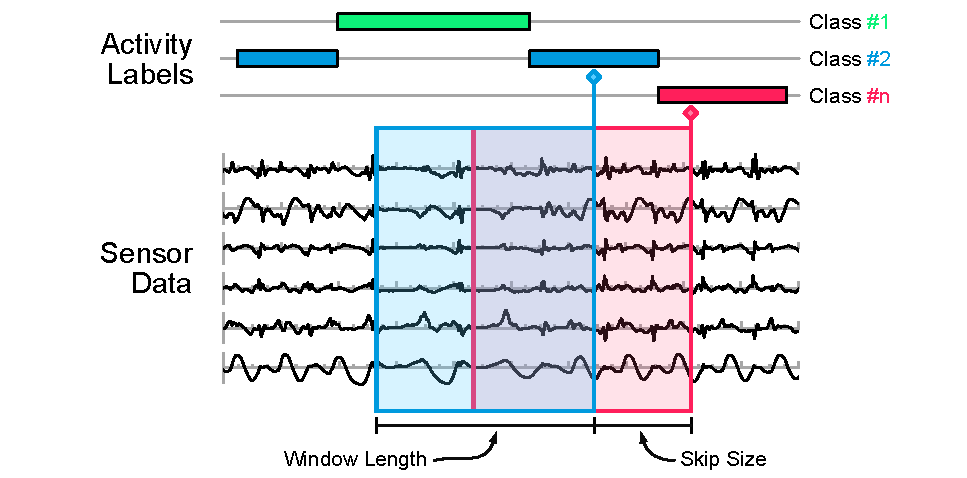
\includegraphics[width=0.9\textwidth]{content/3-Methods/Sliding_Window.pdf}
    \caption{Sliding window generation}
    \label{fig:methods-data-window-generation}
\end{figure}

The activity labels must be provided in the same output scheme as the \acrshort{ml} model, for classification this format is one-hot encoding. Each activity label is represented as an array of length equal to the number of classes. Each element of the array represents one of the classes. To encode the actual class the corresponding array element is given a value of one.

The windowed and labelled data needs to be split into the three data-sets, test, training and validation. How this is achieved will be experiment dependent therefore will be discussed in the methods before each experiment.

\subsubsection{Load}
Finally the three sets of windowed and labelled data are fed into TensorFlow. How TensorFlow is configured to process the transformed data is explained next.


\section{Machine Learning Methods}
TensorFlow and the Keras will be used to develop and evaluate machine learning systems. TensorFlow is an open source platform developed by Google that implements a large number of workflows and tools to develop and deploy machine learning systems. %\cite{https://www.tensorflow.org/ (Accessed 20-01-2022)}
Keras is an abstraction for TensorFlow with a focus on simplifying and optimising the TensorFlow development process. %\cite{https://keras.io/ (Accessed 20-01-2022)}
Within this section the method for generating, training and evaluating model performance will be described.

All machine learning operations were conduced on a desktop Windows PC. The PC was fitted with a Nvidia RTX 2060 super graphics card and a AMD Ryzen 3600 CPU.

% Model generation
All models will be build using the Keras sequential model framework. This allows for the construction models formed of a stack of layers where each layer has exactly one input tensor and one output. tensor.%\cite{https://keras.io/guides/sequential_model/ (Accessed 20-01-2022)}
Greatly simplifying the process of implementing \acrshort{ml} models.

% Training
The generated model can then be trained. Training will be undertaken using the Adam optimiser\cite{Kingma2015}. Two performance metrics will be used to evaluate the training performance. categorical cross-entropy for loss, and categorical accuracy for classification performance. An early stopping scheme will be employed to end training early once training stagnation is detected in the validation data set. Stagnation is detected by a period of worse loss than the best seen.

%Hyper-parameter tuning
Hyper-parameter tuning was achieved through the assignment of values to the large number of model and training parameters were specified as variables. Some hyper-parameters are used to configure the \acrshort{ml} \acrshort{etl}, while others affect the \acrshort{ml} model construction and training. By repeating model construction and training with different hyper-values sensitivities could be evaluated.

\subsection{Performance Analysis}
Final model performance was conducted on the model after training. Performance is evaluated primarily by metrics derived form the classification accuracy of a test data set. Classification accuracy measures the usefulness of a model. Other metrics of performance include the amount of training data required, number epochs to train and size/number of model parameters. These indicate whether a model is feasible to train and deploy.

%How is categorical/classification accuracy calculated
Classification accuracy is calculated by feeding a test set of input into the trained model. The predicted label can then be compared to the real label. The percentage of correct predictions is the classification accuracy.

% Representation as a confusion matrix
This can be broken down further by presenting the number of correct prediction for each class, as well as where mis-classification occurred. This can be done using a confusion matrix. A confusion matrix is a $nxn$ table where is the number of classes. The table columns represent the prediction labels and the rows represent the real labels. Each cell is populated with the number of inputs that were classified for each combination of real and predicted. The main diagonal represents the correct predictions. There are many numeric metrics for evaluating confusion matrices, most commonly Recall, Precision, F1-score.
